% !TeX root = ../main.tex
\section{Измерение коэффициента шума ($K_{\text{ш}}$)}

\subsection{Теоретические сведения и методика проведения измерений}

Коэффициент шума $K_{\text{ш}}$ (Noise Figure, $NF$) является важнейшим показателем качества малошумящих усилителей и определяет меру ухудшения отношения сигнал/шум при прохождении смеси сигнала и шума через исследуемое устройство. 

По определению, коэффициент шума представляет собой отношение реальной спектральной плотности мощности шума на выходе четырехполюсника $G_{\text{вых.реал}}$ к спектральной плотности мощности шума на выходе идеального (нешумящего) усилителя с тем же коэффициентом усиления $K_p$:
\begin{equation}
K_{\text{ш}} = \frac{G_{\text{вых.реал}}}{G_{\text{вых.идеал}}} = \frac{G_{\text{вых.реал}}}{G_0 K_p},
\end{equation}
где $G_0 = k T_0 = -174\text{ дБм/Гц}$ --- спектральная плотность мощности теплового шума согласованного резистивного источника при стандартной температуре $T_0 = 290\text{ К}$ ($k = 1.38 \cdot 10^{-23}\text{ Дж/К}$ --- постоянная Больцмана).

В лабораторных условиях измерение коэффициента шума выполняется косвенным методом с помощью анализатора спектра:
\begin{enumerate}
    \item Вход исследуемого усилителя нагружается на согласованную экранированную нагрузку 50~Ом, являющуюся источником теплового шума с уровнем $G_0$.
    \item Выход усилителя подключается ко входу анализатора спектра через кабель 2 с потерями $IL_2$.
    \item На анализаторе спектра устанавливается полоса пропускания фильтра промежуточной частоты $\text{RBW} = 100\text{ кГц}$ ($\text{RBW}\,[\text{дБГц}] = 10\lg(100 \cdot 10^3) = 50\text{ дБГц}$), включается усреднение по мощности (`Trace: Power Avg`) и внутренний малошумящий предусилитель (`RF Preamp: ON`) для минимизации погрешности от собственных шумов прибора.
    \item Фиксируется уровень интегральной мощности шума $P_{\text{noise}}$ в полосе $\text{RBW}$ на заданной сетке частот.
\end{enumerate}

Расчетная формула для определения коэффициента шума в децибелах с учетом потерь в соединительном кабеле $IL_2$ и коэффициента усиления каскада $K_p = S_{21}$ имеет вид:
\begin{equation}
NF\,[\text{дБ}] = P_{\text{noise}} + IL_2 - (G_0 + 10\lg(\text{RBW}) + K_p),
\end{equation}
где $G_0 = -174\text{ дБм/Гц}$, $10\lg(\text{RBW}) = 50\text{ дБГц}$, а значение $S_{21}$ берется из результатов предыдущего этапа калибровки АЧХ.

\subsection{Результаты экспериментальных исследований}

Экспериментальные данные измерений мощности шума, значения коэффициента усиления и рассчитанные величины коэффициента шума сведены в таблицу~\ref{tab:nf_params}.

\begin{table}[H]
\centering
\caption{Результаты измерений и расчета коэффициента шума усилителя}
\label{tab:nf_params}
\small
\begin{tabular}{|c|c|c|c|c|}
\hline
$f$, МГц & $S_{21}$, дБ & $IL_2$, дБ & $P_{\text{noise}}$, дБм & $NF$, дБ \\
\hline
500  & 23.72 & 0.70 & -98.37 & 2.61 \\
700  & 24.25 & 0.79 & -97.62 & 2.92 \\
1000 & 21.48 & 0.88 & -100.30 & 3.09 \\
1300 & 20.42 & 0.96 & -101.37 & 3.17 \\
1700 & 16.20 & 1.05 & -105.65 & 3.20 \\
2000 & 17.26 & 1.14 & -104.43 & 3.45 \\
2300 & 16.59 & 1.22 & -105.11 & 3.52 \\
2500 & 15.35 & 1.31 & -105.98 & 3.98 \\
2900 & 14.31 & 1.40 & -106.97 & 4.12 \\
\hline
\end{tabular}
\end{table}

По рассчитанным данным построен график частотной зависимости коэффициента шума исследуемого усилителя (рис.~\ref{fig:nf_plot}).

\begin{figure}[H]
    \centering
    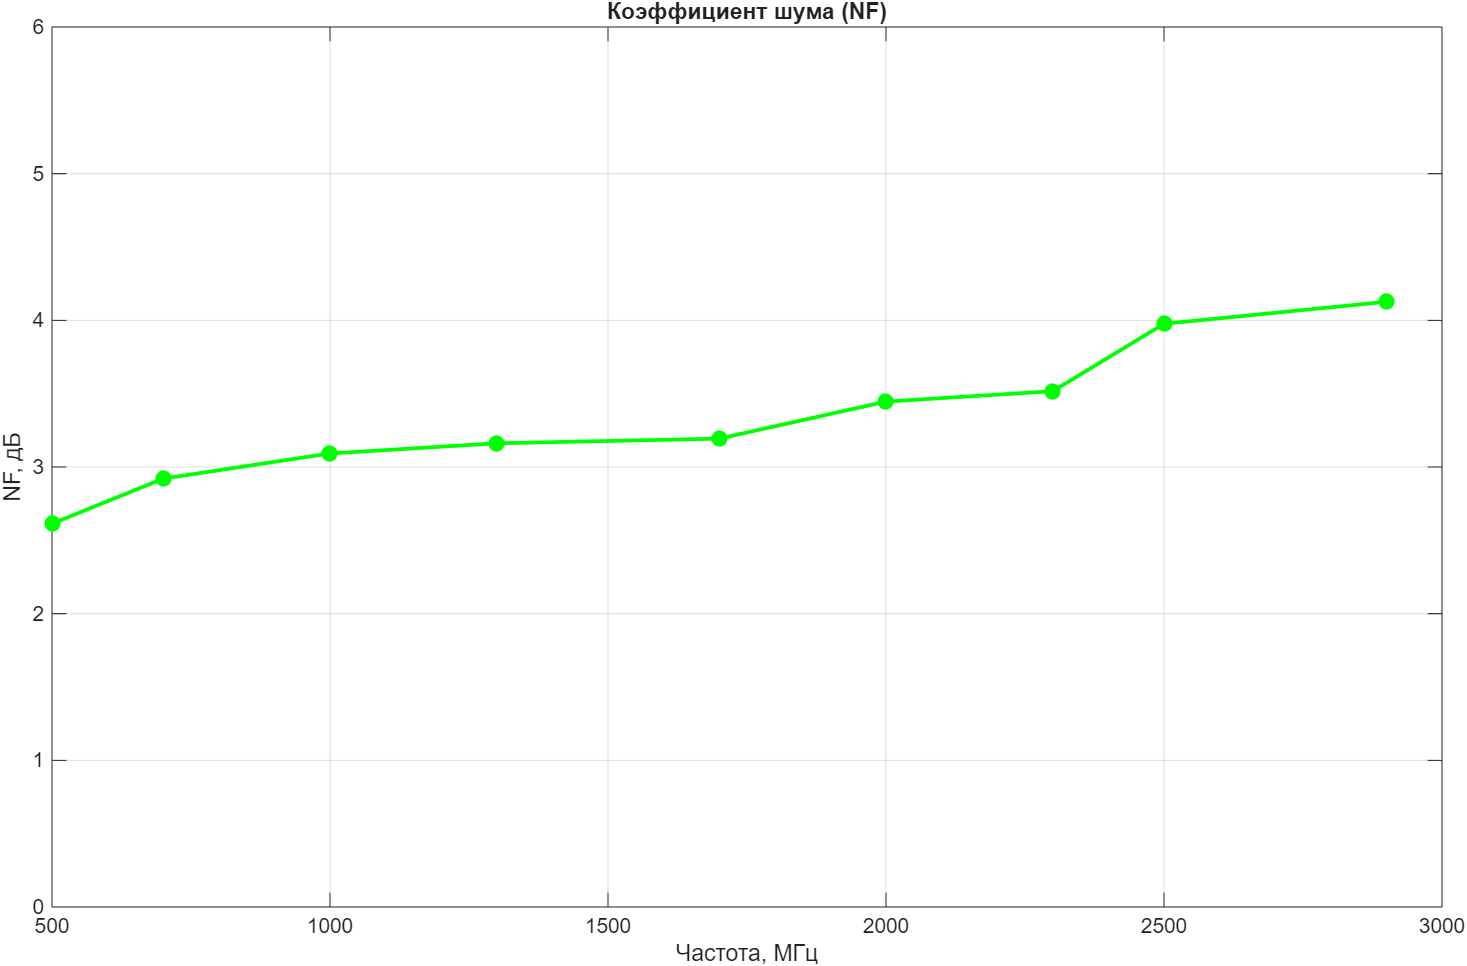
\includegraphics[width=0.88\textwidth]{шум.png}
    \caption{Зависимость коэффициента шума ($NF$) усилителя от частоты}
    \label{fig:nf_plot}
\end{figure}

\subsection{Анализ результатов и выводы}

\begin{enumerate}
    \item \textbf{Шумовые характеристики в полосе пропускания:} В диапазоне частот от 500~МГц до 1700~МГц усилитель демонстрирует хорошие шумовые свойства с низким значением коэффициента шума ($NF \approx 2.6\text{--}3.2\text{ дБ}$). Это подтверждает возможность его эффективного применения в качестве малошумящего входного усилителя (МШУ) радиоприемного тракта дециметрового диапазона волн.
    \item \textbf{Деградация $NF$ на верхних частотах:} При увеличении частоты свыше 1.7~ГГц наблюдается плавный монотонный рост коэффициента шума, достигающего значения $4.12\text{ дБ}$ на частоте 2900~МГц. Ухудшение шумовых свойств усилителя на СВЧ вызвано возрастанием вклада высокочастотных шумов транзистора (теплового шума распределенного сопротивления базы, фликкер-эффекта и пролетных явлений), а также спадом коэффициента усиления $S_{21}$, из-за чего собственный шум последующих каскадов и цепей согласования слабее ослабляется в пересчете ко входу.
    \item \textbf{Влияние измерительного тракта:} Учет затухания соединительного кабеля ($IL_2$ от 0.70 до 1.40~дБ) и нормировка на эффективную полосу пропускания фильтра ПЧ анализатора спектра ($10\lg(\text{RBW}) = 50\text{ дБ}$) позволили исключить систематические ошибки прибора и получить достоверную физическую величину шумовой меры самого полупроводникового каскада.
\end{enumerate}